% ****** Start of file apssamp.tex ******
%
%   This file is part of the APS files in the REVTeX 4.1 distribution.
%   Version 4.1r of REVTeX, August 2010
%
%   Copyright (c) 2009, 2010 The American Physical Society.
%
%   See the REVTeX 4 README file for restrictions and more information.
%
% TeX'ing this file requires that you have AMS-LaTeX 2.0 installed
% as well as the rest of the prerequisites for REVTeX 4.1
%
% See the REVTeX 4 README file
% It also requires running BibTeX. The commands are as follows:
%
%  1)  latex apssamp.tex
%  2)  bibtex apssamp
%  3)  latex apssamp.tex
%  4)  latex apssamp.tex
%
\documentclass[%
reprint,
%superscriptaddress,
%groupedaddress,
%unsortedaddress,
%runinaddress,
%frontmatterverbose, 
%preprint,
%showpacs,preprintnumbers,
%nofootinbib,
%nobibnotes,
%bibnotes,
 amsmath,amssymb,
 aps,
%linenumbers,
%pra,
%prb,
%rmp,
%prstab,
%prstper,
%floatfix,
]{revtex4-1}

\usepackage{graphicx}% Include figure files
\usepackage{dcolumn}% Align table columns on decimal point
\usepackage{bm}% bold math
%\usepackage{hyperref}% add hypertext capabilities
%\usepackage[mathlines]{lineno}% Enable numbering of text and display math
%\linenumbers\relax % Commence numbering lines

%\usepackage[showframe,%Uncomment any one of the following lines to test 
%%scale=0.7, marginratio={1:1, 2:3}, ignoreall,% default settings
%%text={7in,10in},centering,
%%margin=1.5in,
%%total={6.5in,8.75in}, top=1.2in, left=0.9in, includefoot,
%%height=10in,a5paper,hmargin={3cm,0.8in},
%]{geometry}


%%%%%%%%%%%%%%%%%%%%%%%%%%%
%%%%%%  PREAMBLES %%%%%%%%%
\newcommand{\ud}[1]{{#1^{\dagger}}}
\newcommand{\bra}[1]{\left\langle #1\right|}
\newcommand{\ket}[1]{\left| #1\right\rangle}
\newcommand\Tr{\mathrm{Tr}}
\newcommand{\braket}[2]{\langle #1 \mid #2 \rangle}
\newcommand\I{\mathbb{I}}
\newcommand{\avg}[1]{\left< #1 \right>}
\newcommand{\sech}[1]{{\operatorname{sech}{#1}}}
\newcommand{\csch}[1]{{\operatorname{csch}{#1}}}
%%%%%%  PREAMBLES %%%%%%%%%
%%%%%%%%%%%%%%%%%%%%%%%%%%%

\begin{document}

%\preprint{APS/123-QED}

\title{Parametric neutrino flavor conversion and Rabi oscillation}% Force line breaks with \\
%\thanks{A footnote to the article title}%

\author{Lei Ma}
\email{leima@unm.edu}
\author{Shashank Shalgar}%
\email{shashankshalgar@unm.edu}
\author{Huaiyu Duan}%
\email{duan@unm.edu}
\affiliation{%
 Department of Physics \& Astronomy, University of New Mexico,
 Albuquerque, NM 87131, USA
}%
% \author{Huaiyu Duan}%
%  \email{Second.Author@institution.edu}
% \affiliation{%
%  Authors' institution and/or address\\
%  This line break forced with \textbackslash\textbackslash
% }%

% \collaboration{MUSO Collaboration}%\noaffiliation

% \author{Shashank Shalgar}
%  \homepage{http://www.Second.institution.edu/~Charlie.Author}
% \affiliation{
%  Second institution and/or address\\
%  This line break forced% with \\
% }%
% \affiliation{
%  Third institution, the second for Charlie Author
% }%
% \author{Delta Author}
% \affiliation{%
%  Authors' institution and/or address\\
%  This line break forced with \textbackslash\textbackslash
% }%

% \collaboration{CLEO Collaboration}%\noaffiliation

% \author{Huaiyu Duan}
%  \homepage{http://www.Second.institution.edu/~Charlie.Author}
% \affiliation{
%  Second institution and/or address\\
%  This line break forced% with \\
% }%
% \affiliation{
%  Third institution, the second for Charlie Author
% }%
% \author{Delta Author}
% \affiliation{%
%  Authors' institution and/or address\\
%  This line break forced with \textbackslash\textbackslash
% }%

% \collaboration{CLEO Collaboration}%\noaffiliation



\date{\today}% It is always \today, today,
             %  but any date may be explicitly specified

\begin{abstract}
\fbox{ABSTRACT PLACEHOLDER}
% \begin{description}
% \item[Usage]
% Secondary publications and information retrieval purposes.
% \item[PACS numbers]
% May be entered using the \verb+\pacs{#1}+ command.
% \item[Structure]
% You may use the \texttt{description} environment to structure your abstract;
% use the optional argument of the \verb+\item+ command to give the category of each item. 
% \end{description}
\end{abstract}

% \pacs{Valid PACS appear here}% PACS, the Physics and Astronomy
                             % Classification Scheme.
%\keywords{Suggested keywords}%Use showkeys class option if keyword
                              %display desired
\maketitle

%\tableofcontents

\section{\label{introduction}Introduction}

In many astrophysical environments, such as core-collapse supernova,  neutrinos propagate through dense fluctuating medium, which will interact with neutrinos and dramatically change the flavor oscillations of neutrinos. The significance of matter effect on neutrino flavor oscillations has been demonstrated in Mikheyev–-Smirnov–-Wolfenstein (MSW) effect, which is used to explain the deficit of electron flavor neutrino flux, thus solved the solar neutrino problem~\cite{wolf78,Petcov2002}. Another matter effect of interest is parametric resonance of neutrino flavor oscillations due to fluctuations in matter~\cite{Krastev1989,Akhmedov2000}. Recently matter stimulated neutrino flavor conversion in varying matter density has been researched using Jacobi-Anger expansion by Kneller, et al.~\cite{Kneller2013,Patton2014}. They have shown that many stimulated neutrino oscillations can be explained by resonances of the system. 

In this manuscript, we take a step further and interpret parametric resonance~\cite{Akhmedov2000, Krastev1989} as well as other stimulated neutrino oscillations~\cite{Kneller2013, Patton2014}, as superpositions of Rabi oscillations. In Sec.~\ref{sec:background}, we define the formalism of neutrino oscillations in matter used in this paper. In Sec.~\ref{sec:simple} we discuss how neutrino oscillations are related to Rabi oscillations by dropping less important terms. In Sec.~\ref{sec:jacobi} we discuss the technique of decomposing the neutrino oscillation system into Rabi oscillations, by applying a specific unitary transformation and the Jacobi-Anger expansion.


\fbox{TODO:more about oscillation in matter}

\section{\label{sec:background}Background and Formalism}

\fbox{TODO: Explain why two flavor}

We consider two-flavor oscillation scenario, in which neutrinos have energy $E$ and mass-squared difference $\delta m^2$ between two mass states propagate through matter which is define by electron number density profile $n(r)$ along the path of neutrino propagation $r$. Three different bases are used in this work, i.e., flavor basis, in which the wave function describes the probability amplitude of different flavors, background matter basis, in which the wave function describe the probability amplitude of different mass states with the appearance of only background matter density, and Rabi basis which will be defined explicitly later. These different bases are also defined in Appendix~\ref{sec:three-bases}. The dynamics of neutrino flavor conversion is determined by Schr\"{o}dinger equation, in which the Hamiltonian in flavor basis is
\begin{equation}
    H^{(\mathrm{f})} =  \frac{1}{2} \begin{pmatrix}
    -\omega_{\mathrm{v}} \cos 2\theta_{\mathrm{v}} + \lambda(r) & \omega_{\mathrm{v}}\sin 2\theta_{\mathrm{v}} \\
   \omega_{\mathrm{v}} \sin 2\theta_{\mathrm{v}} & \omega_{\mathrm{v}} \cos 2\theta_{\mathrm{v}} - \lambda(r)
    \end{pmatrix},
\end{equation}
where $\lambda(r)= \sqrt{2}G_F n(r)$ is the potential due to neutrino interaction with matter and $G_F$ is the Fermi constant, $\theta_{\mathrm{v}}$ is the vacuum mixing angle, $\omega_{\mathrm{v}} = \delta m^2/2E$ is the vacuum oscillation frequency. For the convenience of notation, we use Pauli matrices $\sigma_i$ to denote the Hamiltonian, so that the Schr\"{o}dinger equation becomes,
\begin{equation}
    \mathrm i\frac{\mathrm d}{\mathrm d r}\Psi(r) = \frac{1}{2} \left(  
    (- \omega_{\mathrm{v}}\cos 2\theta_{\mathrm{v}} + \lambda(r) ) \sigma_3 + \omega_{\mathrm{v}}\sin 2\theta_{\mathrm{v}} \sigma_1 
    \right)
    \Psi(r),
\end{equation}
where $\Psi(r)$ is the wave function in flavor basis. For two flavor system, it is written as $ \Psi(r) = \left(
    \psi_{e} ,
    \psi_{x}
    \right)^{\mathrm{T}}$ 
where $\psi_{e}$ and $\psi_{x}$ are the amplitudes for electron flavor and the second flavor ($\mu$ flavor or $\tau$ flavor) respectively. The equation of motion in flavor basis reveals the transitions between different flavors directly.


The potential $\lambda(r)$ for a general perturbation on top of a constant matter profile can be written as
\begin{equation}
    \lambda(r) = \lambda_0 + \delta \lambda(r).
    \label{eq-general-matter-profile}
\end{equation}
For better understanding of the transition between states due to the effect of matter, we use the background matter basis, in which the Hamiltonian is diagonalized in the absence of perturbation $\delta\lambda(r)$, so that the Hamiltonian becomes
\begin{widetext}
\begin{equation}
    H^{(\mathrm{m})} = -\frac{\omega_m}{2} \sigma_3 + \frac{1}{2} \delta\lambda(r) \cos 2\theta_{\mathrm m} \sigma_3 
     - \frac{1}{2} \delta\lambda(r) \sin 2\theta_{\mathrm m} \sigma_1,
    \label{eq-hamiltonian-bg-matter-basis-general}
\end{equation}
\end{widetext}
where $\theta_{\mathrm m}$ is the mixing angle in a constant matter profile $\lambda_0$, which is calculated using relation
\begin{equation*}
\tan 2\theta_{\mathrm{m}}=\sin 2\theta_{\mathrm v}/\left( \cos 2\theta_{\mathrm v} - \lambda_0/\omega_{\mathrm v} \right)
\end{equation*}
with $\omega_{\mathrm v}$ denoting the vacuum oscillation frequency and $\theta_{\mathrm v}$ denoting the vacuum mixing angle. The energy split is defined as
\begin{equation}
\omega_{\mathrm{m}} = \omega_{\mathrm{v}} \sqrt{ ( \lambda_0/\omega_{\mathrm{v}} - \cos (2\theta_{\mathrm{v}}) )^2 + \sin^2(2\theta_{\mathrm{v}}) }.
\end{equation}




%%%%%%%%%%%%%%%%%%%%%%%%%%%%%%%%%%%%%%%%%%%%%%%%%%%%
%% Simplified Model
%%%%%%%%%%%%%%%%%%%%%%%%%%%%%%%%%%%%%%%%%%%%%%%%%%%%

\section{\label{sec:simple}Parametric Resonance and Rabi oscillation --- a simplified model}%


In this section we present a simple picture to explain neutrino parametric resonance in matter by utilizing the theory of Rabi oscillations. Rabi oscillations have been well studied in quantum optics.\cite{Boyd2008} In Appendix~\ref{sec:rabi-oscillations}, we derive the Rabi oscillation transition probabilities using neutrino flavor isospin method introduced in Ref.~\onlinecite{Duan2006a}.




%%%%%%%%%%%%%%%%%%%%%%%%%%%%%%%%%%%%
%%%%%%%%% Rabi oscillation
%%%%%%%%%%%%%%%%%%%%%%%%%%%%%%%%%%%%


% The Hamiltonian Eq.~\ref{eq-hamiltonian-bg-matter-basis-general} has a lot in common with the Rabi oscillation Hamiltonian. One example of Rabi oscillation is the transition between low energy state and high energy state in two level atoms, when stimulated by optical fields with frequency that matches the energy gap of the two level atoms. As the frequency of optical field approaches the energy split of atom, large transition occurs, which is described by Rabi formula. 

% In the light of Rabi oscillations, we argue that the second term in the neutrino system described by Eq.~(\ref{eq-hamiltonian-bg-matter-basis-general}), i.e., the varying diagonal elements of Hamiltonian, is not relevant when the system is close to resonance, as we will explain later using Jacobi-Anger expansion. 


\subsection{\label{sec:single-freq}Single Frequency Matter Profile}


The first example we examine is single frequency matter profile $\delta\lambda(r) = \lambda_1 \sin(k_1 r)$. As proved later, the varying $\sigma_3$ term $\delta\lambda(r) \cos 2\theta_{\mathrm m} \sigma_3/2$ in Hamiltonian Eq.~(\ref{eq-hamiltonian-bg-matter-basis-general}) has little effect on the transition probabilities when the system is close to resonance. With the varying $\sigma_3$ term removed, it indicates that this single frequency matter perturbation neutrino oscillation system is a Rabi oscillation system, with external driving field frequency $k_1$ and energy gap $\omega_{\mathrm m}$. By dropping the off resonance terms, the Hamiltonian is simplified to
% \begin{align}
% H^{(\mathrm{m})}_1 &= -\frac{\omega_{\mathrm m}}{2} \sigma_3 + \frac{1}{2} \lambda_1 \sin(k_1 r) \cos 2\theta_{\mathrm m} \sigma_3 -\frac{1}{2}\lambda_1 \sin(k_1 r) \sin 2\theta_{\mathrm m} \sigma_1 \\
% &\to -\frac{\omega_{\mathrm m}}{2} \sigma_3  -\frac{1}{2}\lambda_1 \sin(k_1 r) \sin 2\theta_{\mathrm m} \sigma_1,
%     \label{eq-hamiltonian-bg-matter-basis-single-frequency}
% \end{align}
\begin{align}
H^{(\mathrm{m})} \to & -\frac{\omega_{\mathrm m}}{2} \sigma_3  - \frac{1}{2} \lambda_1 \sin 2\theta_{\mathrm m} \sin( k_1 r ) \sigma_1 \\
\to & -\frac{\omega_{\mathrm m}}{2} \sigma_3  - \frac{1}{2} A_1 \cos ( k_1 r)  \sigma_1 + \frac{1}{2} A_1\sin(k_1 r) \sigma_2,\nonumber 
    \label{eq-hamiltonian-bg-matter-basis-single-frequency}
\end{align}
where
\begin{equation}
A_1 = \frac{\lambda_1 \sin 2\theta_{\mathrm m} }{2i}.
\end{equation}

The resonance condition is determined by matching the energy gap $\omega_{\mathrm m}$ with external driving field frequency $k_1$, i.e., $\omega_{\mathrm m} \sim k_1$. As the condition is approaching resonance condition, the transition probability is predicted well using Rabi formula.

% For a graphical representation of such resonances, decompositions of Hamiltonian onto Pauli matrices are denoted as vectors on , c.f.~Appendix~\ref{sec:rabi-oscillations}. The Hamiltonian is decomposed into three different components, i.e., the constant energy gap on z axis $\vec H_z$, the varying perturbation on z axis $\vec H_{z}'$, and the rotating perturbations in xy plane $\vec H_{\pm}$. The frequency of the rotating component $H_{+}$ in the xy can easily match the energy gap $\omega_{\mathrm{m}}$ even with a varying $\vec H_z'$ component in the Hamiltonian vector, as long as the system is close to resonance.

To show that this conjecture is correct, we calculate transition probabilities of the neutrinos described by Eq.~(\ref{eq-hamiltonian-bg-matter-basis-general}), and the Rabi oscillations described by Eq.~(\ref{rabi-oscillation-single-perturbation}), with parameters chosen so that the two systems have the same energy split and driving field strength and frequency. In FIG.~\ref{fig-rabiOscillationsNeutrinoCoincidence}, black dots show the transition probability of neutrino oscillation in matter, while solid line stands for the result predicted using Rabi formula.

For a single frequency perturbation in matter profile $\lambda(r) =\lambda_1 +  \lambda_1\sin(k_1 r)$, P. Krastev and A. Smirnov concluded that the parametric resonance condition is $\omega_{\mathrm{m}} \sim n k_1$, if instantaneous $\omega_{\mathrm{m,inst}}(r)$ associated with the matter profile at distance $r$ varies slowly~\cite{Krastev1989}. This condition is exactly the Rabi resonance condition when $n=1$, as such condition matches the driving field frequency to the energy split.





\begin{figure}[!htbp]
                \centering
                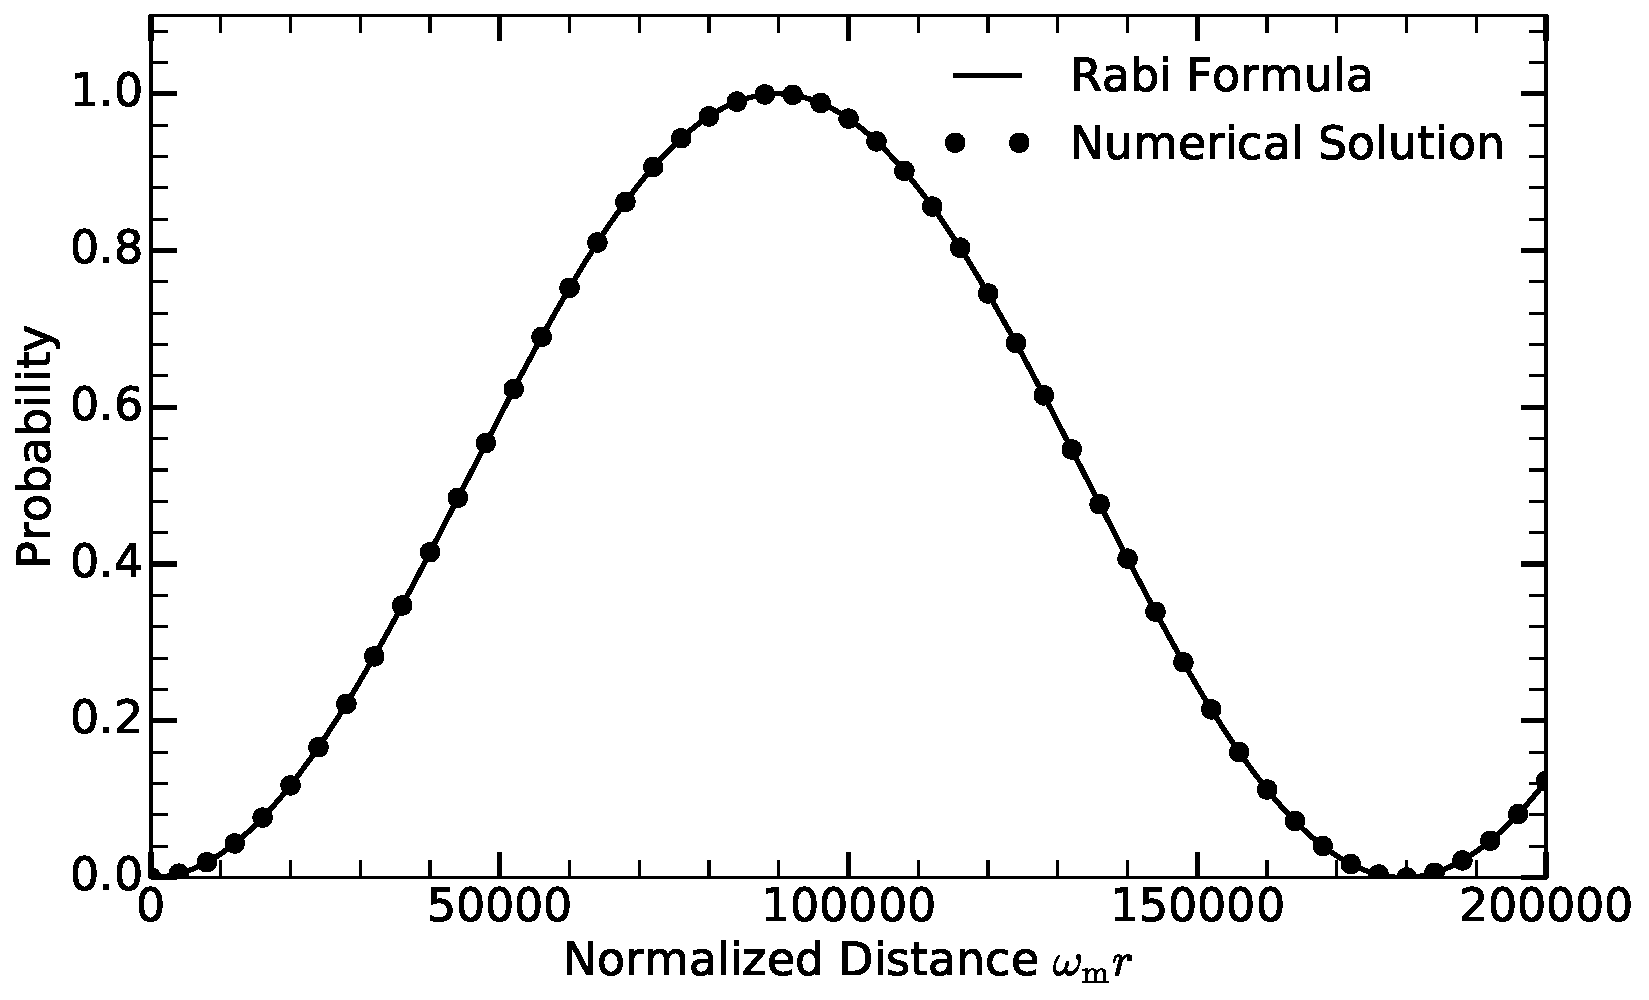
\includegraphics[width=\columnwidth]{assets/rabiOscillationsNeutrinoCoincidence-single-frequency}
                %rabiOscillationsNeutrinoCoincidence}
                \caption{Single frequency matter profile and Rabi oscillation.  Black dots are the transition probabilities between two background mass eigenstates for the neutrinos with matter perturbation $A_1\sin(k_1 r)$. During the calculation, $\lambda_0$ is set to $0.5$ of the MSW resonance potential $\lambda_{\mathrm{MSW}}=\omega_{\mathrm{v}}\cos 2\theta_{\mathrm v}$ and mixing angle is chosen so that $\sin^2(2\theta_{\mathrm v}) = 0.093$. The solid line is the probabilities predicted using Rabi formula.}
                \label{fig-rabiOscillationsNeutrinoCoincidence}
\end{figure}






\subsection{Castle Wall Matter Profile}

The approach applied to single frequency matter profile also helps with the understanding of multiple frequency matter profile. Since any matter profile can be Fourier decomposed into superposition of many single frequency matter profile, we show an example of another well studied matter profile which is the periodic castle wall matter profile. The potential shown in Fig.~\ref{fig-castlewall-profile-illustration} is defined as,
\begin{equation}
    \lambda(r) = \begin{cases} 
\Lambda_1, &\quad -\frac{X_1}{2}+nX\le r\le \frac{X_1}{2}+nX \\
\Lambda_2, &\quad \frac{X_1}{2}+nX\le r\le \frac{X_1}{2}+\frac{X_2}{2} +nX
\end{cases}
\label{eq-castle-wall-potential}
\end{equation}
where $X_1$ and $X_2$ are the two periods of the matter profile or potential, $X=X_1+X_2$, and $n$ is integer. The parametric resonance condition derived by E. Akhmedov~\cite{Akhmedov2000} is,
\begin{equation}
    \frac{\tan (\omega_{\mathrm m1}X_1/2)}{\tan (\omega_{\mathrm m2}X_2/2)} = - \frac{\cos 2\theta_{\mathrm m2}}{\cos 2\theta_{\mathrm m1}},
\end{equation}
where $\omega_{\mathrm{m}i}$ and $\theta_{\mathrm{m}i}$ are the energy difference and mixing angle for potential $\Lambda_1$ and $\Lambda_2$ respectively.

\begin{figure}
    \centering
    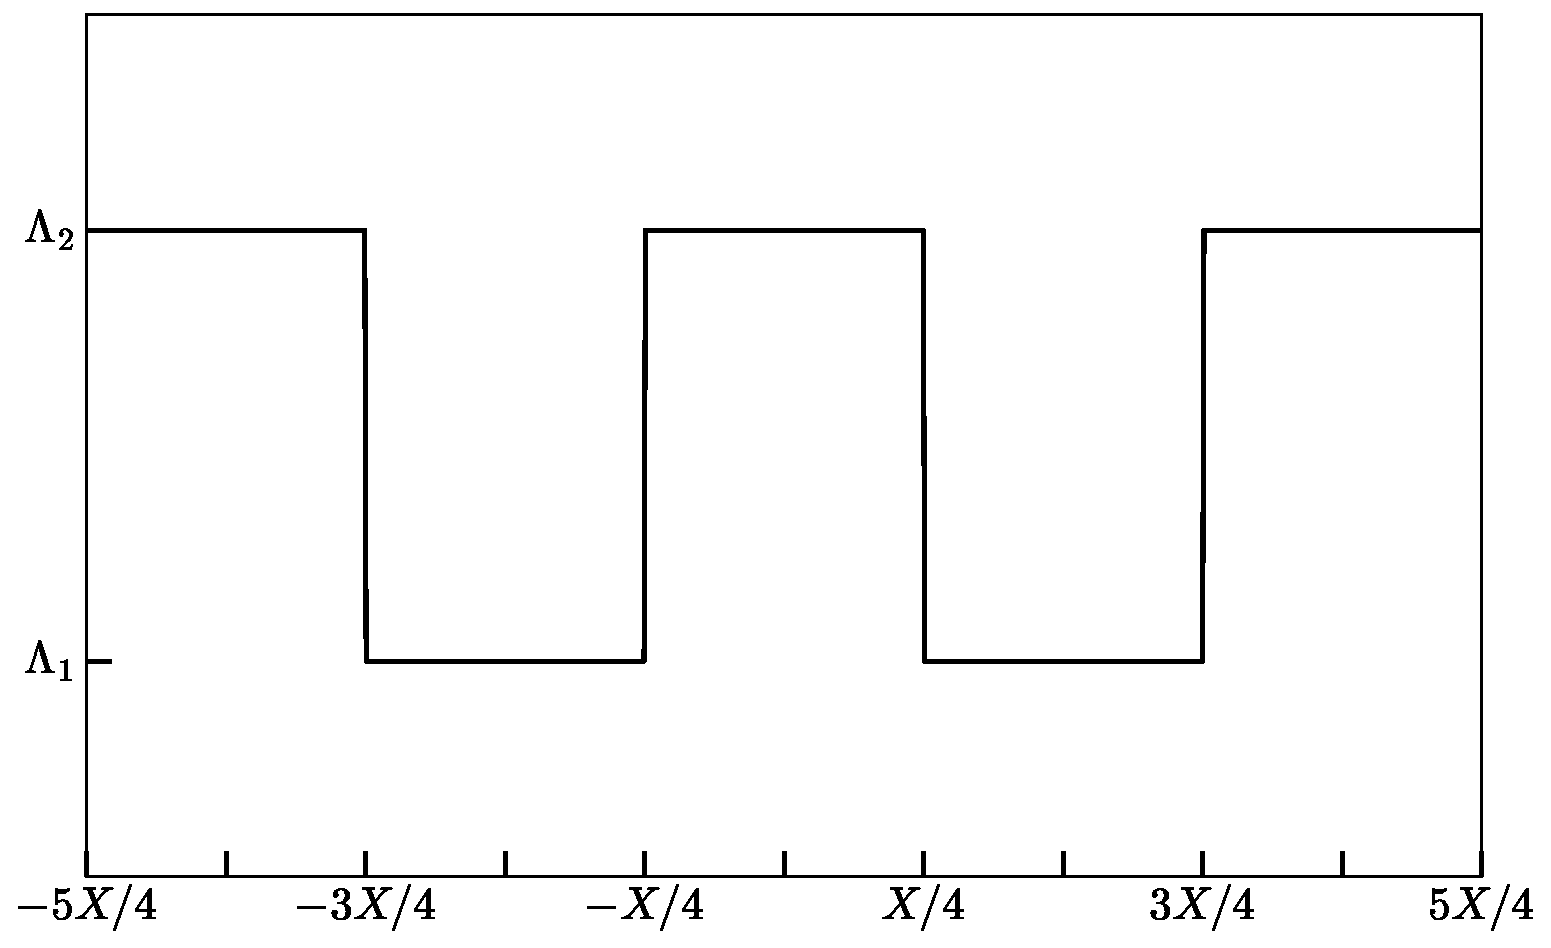
\includegraphics[width=\columnwidth]{assets/castlewall-profile}
    \caption{The castle wall matter potential profile with $X_1=X_2=X/2$.}
    \label{fig-castlewall-profile-illustration}
\end{figure}

Even though this castle wall problem is exactly solved, the condition itself is not transparent. In this subsection, we show that such a system is closed related to Rabi oscillations by making appropriate approximation, which will be be specifically proved in Sec.~\ref{sec:jacobi}.

For illustration purpose, we set the profile to be equal period for the two densities so that $X_1=X_2\equiv X/2$. To show that the neutrino transitions in this castle wall matter profiles is related to Rabi oscillation, we decompose the profile using Fourier series,
\begin{equation}
\lambda(r) = \lambda_0 + \sum_{n=1}^{\infty} \lambda_n \cos\left( k_n  r \right),
\end{equation}
where 
\begin{align*}
\lambda_0 &= (\Lambda_1 + \Lambda_2)/2, \\
\lambda_n & = \frac{2}{(2n-1)\pi}  (-1)^n  \left( \Lambda_1 -  \Lambda_2 \right),\\
k_n &= (2n-1)k_0, \\
k_0 &= 2\pi/X.
\end{align*}

To calculate the transitions between two mass states of background matter potential $\lambda_0$, we rotate to the background matter basis with respect to $\lambda_0$, in which the transition is zero when variations of matter profile vanishes. The Hamiltonian
\begin{widetext}
\begin{equation}
H^{(\mathrm m)} = - \frac{1}{2}\omega_{\mathrm m} \sigma_3  + \frac{1}{2} \sum_{n=1}^{\infty} \lambda_n \cos 2\theta_{\mathrm m} \cos\left( k_n  r \right)  \sigma_3 - \frac{1}{2} \sum_{n=1}^{\infty} \lambda_n \sin 2\theta_{\mathrm m}  \cos\left( k_n r \right) \sigma_1,
\label{castle-wall-decomposed-hamiltonian}
\end{equation}
\end{widetext}
determines the transitions between the two background matter states.


\begin{figure}[!htbp]
                \centering
                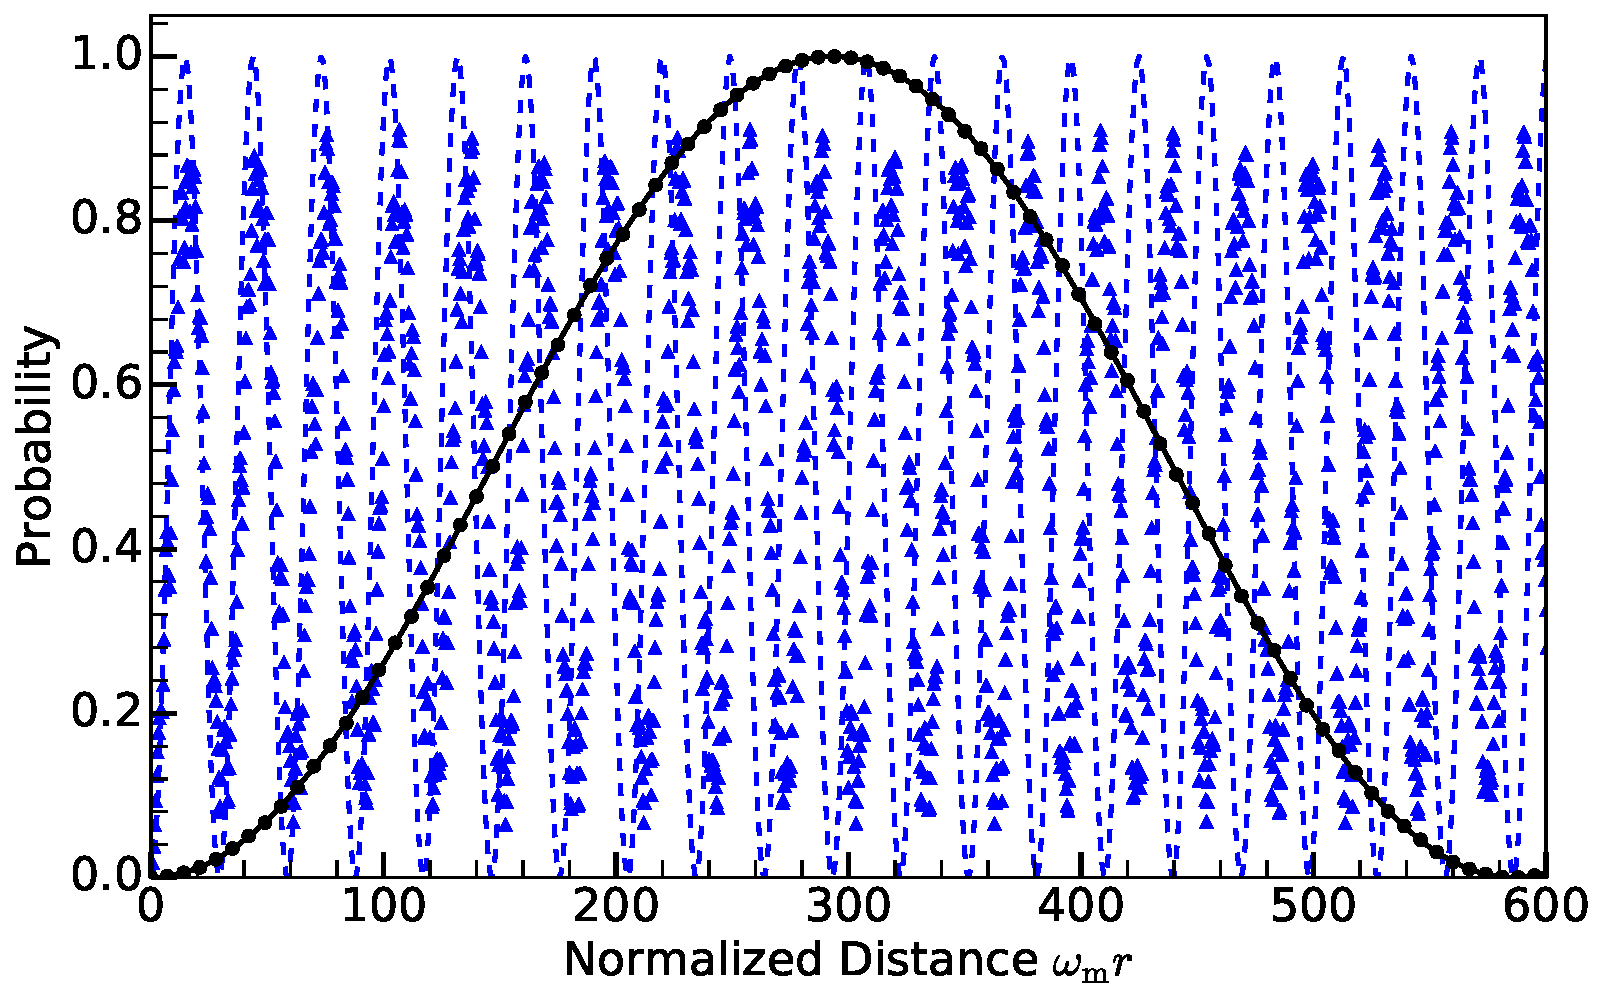
\includegraphics[width=\columnwidth]{assets/castle-wall}
                \caption{Transition probabilities for castle wall matter profile. 
                %The black solid line is the transition probabilities for $\lambda_2-\lambda_1=0.09\lambda_0$ calculated using Rabi formula, while black dots are the numerical solution; The red dashed line is the transition probabilities for $\lambda_2-\lambda_1=0.1\lambda_0$ calculated using Rabi formula, while red up-pointing triangles are the numerical solution; The blue dash-dotted line is the transition probabilities for $\lambda_2-\lambda_1=0.2\lambda_0$ calculated using Rabi formula, while blue down-pointing triangles are the numerical solution. 
                The black dots, and blue triangles are the transition probabilities of castle wall matter profile calculated numerically for $\Lambda_2-\Lambda_1=0.04\Lambda_0$, and $\Lambda_2-\Lambda_1=0.8\Lambda_0$ respectively, while the black solid line, and blue dashed line are the corresponding Rabi formula. During the calculation, the energy of neutrinos is $10\,\mathrm{MeV}$, mass-squared difference is $\delta m^2=2.6\times 10^{-3}\,\mathrm{eV^2}$, and the vacuum mixing angle chosen so that $\sin^2(2\theta_v)=0.093$. The background potential $\Lambda_0$ is chosen so that it's half the MSW resonance potential, $\Lambda_0 = \frac{1}{2}\lambda_{\mathrm{MSW}}=\frac{1}{2}\omega_{\mathrm{v}}\cos 2\theta_{\mathrm v}$, and the base frequency is set to $k_0 = 2\pi/X = \omega_{\mathrm{m}}$.
                }
                \label{fig-akhmedovOscPlt}
\end{figure}


In principle, the base frequency $k_0$ which is determined by the total period $X$ can be arbitrary. In this example, we choose a proper $X$ so that the base frequency $k_0$ matches the energy gap $\omega_{\mathrm{m}}$. Even though multiple perturbations frequencies show up in Eq.~(\ref{castle-wall-decomposed-hamiltonian}), we identify that only the first mode is the resonance mode due to the value we choose. As an estimation, we drop all other modes. Thus, similar to single frequency matter profile, the varying $\sigma_3$ terms have limited effects on the transition probabilities when the system is close to resonance, so that
\begin{align*}
    H^{(\mathrm m)} \to & - \frac{1}{2}\omega_{\mathrm m} \sigma_3  - \frac{1}{2} \lambda_1 \sin 2\theta_{\mathrm m}  \cos\left( k_0 r \right) \sigma_1\\
    \to & - \frac{1}{2}\omega_{\mathrm m} \sigma_3  - \frac{1}{2} A_1 \cos ( k_0 r) \sigma_1 + \frac{1}{2} A_1 \sin(k_0 r) \sigma_2,
\end{align*}
where
\begin{equation*}
A_1 = \frac{\lambda_1 \sin 2\theta_{\mathrm m} }{2} .
\end{equation*}


FIG.~\ref{fig-akhmedovOscPlt} shows the neutrino transitions between the two matter states for different $\Lambda_2-\Lambda_1$. For small $\Lambda_2-\Lambda_1$, the Rabi formula prediction using the resonance mode $k_0$ only matches the numerical results. The reason is that the resonance width of each mode is small, so that the interference between the resonance mode and all other modes are small. We notice larger deficit between Rabi formula predictions and numerical results for large $\Lambda_2-\Lambda_1$, which is due to the destruction effect of the interference with between modes.






%%%%%%%%%
%%%% Interference
%%%%%%%%


\subsection{Interference with Long Wave Length Mode}

% \fbox{
% \parbox{0.9\columnwidth}{
% \begin{itemize}
%     \item Two limits: strong interference regime and low-interference regime
%     \item For strong interference we include multiple modes
%     \item For weak interference, we can interpret the case that one of the matter profile wavelength is much larger than the other. In this case we have a shift of background matter density of the short wavelength perturbation profile.
%     \item Examples. A slight shift in the background density could remove the resonance, which can be quantified.
%     \begin{equation*}
%         a
%     \end{equation*}
% \end{itemize}
% }
% }


The interference effect between different modes in multiple frequency Rabi oscillations can be illustrated using a two-mode model. In Fig.~\ref{fig-akhmedovOscPlt}, the transition amplitude drops for larger fluctuations $\Lambda_2-\Lambda_1$. Such destruction effect can be interpreted as shift of energy gap due to the long wavelength perturbation. To model the effect, we construct a Rabi oscillation Hamiltonian with two modes of different frequency,
\begin{widetext}
\begin{equation}
H^{(\mathrm{m})}  = -\frac{\omega_{\mathrm{m}}}{2} \sigma_3 - \frac{1}{2} \sum_{n=1}^2  A_n \cos (k_n r) \sigma_1 + \frac{1}{2} \sum_{n=1}^2  A_n \sin (k_n r) \sigma_2 .
\label{eq-hamiltonian-rabi-two-modes-interference}
\end{equation}
\end{widetext}

To show the destruction effect, the Hamiltonian Eq.~(\ref{eq-hamiltonian-rabi-two-modes-interference}) is written as vectors with sigma matrices as the basis,
\begin{equation}
\mathbf H = \begin{pmatrix}
0\\
0\\
\omega_m
\end{pmatrix} + \begin{pmatrix}
A_1 \cos (k_1 r)\\
-A_1 \sin (k_1 r)\\
0
\end{pmatrix} + \begin{pmatrix}
A_2 \cos (k_2 r)\\
-A_2 \sin (k_2 r)\\
0
\end{pmatrix}.
\end{equation}

The three terms are defined as $\mathbf  H_3$, $\mathbf H_1$, and $\mathbf H_2$, where $\mathbf H_3$ is perpendicular to the other two vectors. Assuming $\mathbf H_2$ is the slow rotating field, i.e., $k_2<k_1$, the shift of energy gap is calculated as
\begin{align}
    \omega_{\mathrm{m}}' =& \sqrt{\omega_{\mathrm{m}}^2 + A_2^2 } \\
    \approx & \omega_{\mathrm{m}} + \frac{A_2^2}{2\omega_{m}},
\end{align}
where we keep only first order of Taylor series.
    
To begin with, the first rotating perturbation satisfies the resonance condition $k_1=\omega_{\mathrm{m}}$, the condition for the second slow rotating field shifting the system out of resonance is that the detuning becomes larger than the resonance width,
\begin{equation}
\lvert \omega_{\mathrm{m}}' - \omega_{\mathrm{m}} \rvert \geq A_1,
\end{equation}
which leads to
\begin{equation}
A_2 \geq \sqrt{2\omega_{\mathrm{m}}A_1} \equiv A_{2,\mathrm{Critical}}.
\end{equation}


\begin{figure}[!htbp]
                \centering
                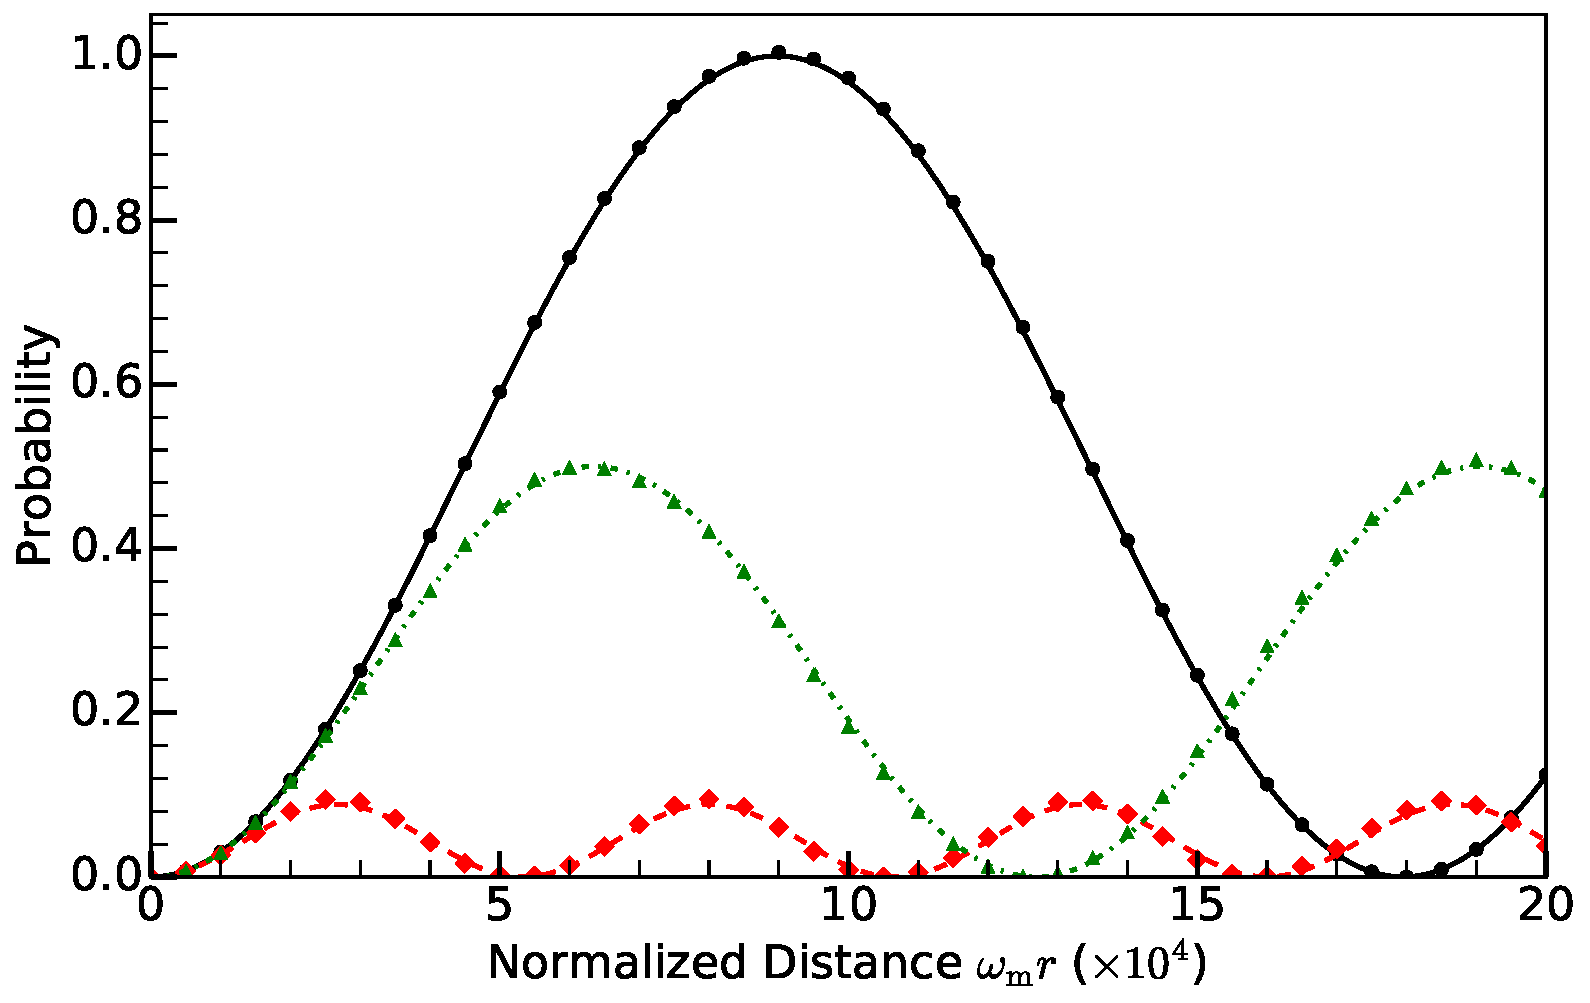
\includegraphics[width=\columnwidth]{assets/interference-reduction}
                \caption{Reduction of transition amplitudes. Black dots are the numerical transition amplitudes for only one mode perturbation which is at resonance, i.e., $A_1=0.000035\omega_{\mathrm m}$, $k_1=\omega_{\mathrm m}$; Green diamonds are the numerical transition amplitude with a second mode, $A_2=A_{2,\mathrm{Critical}}=0.0083666\omega_{\mathrm m}$, $k_2=0.01\omega_{\mathrm m}$; Red up-pointing triangles are the numerical transition amplitudes with a second mode, $A_2=0.01\omega_{\mathrm m}$, $k_2=0.01\omega_{\mathrm m}$; Blue down-pointing triangles  the numerical transition amplitudes with a second mode, $A_2=0.02\omega_{\mathrm m}$, $k_2=0.01\omega_{\mathrm m}$. The lines are the probabilities predicted using Rabi formula correspondingly. During the calculation, $\Lambda_0$ is set to half of the MSW resonance potential, $\Lambda_0 = \frac{1}{2}\lambda_{\mathrm{MSW}}=\frac{1}{2}\omega_{\mathrm{v}}\cos 2\theta_{\mathrm v}$.}
                \label{fig-rabi-oscillations-energy-gap-change}
\end{figure}


We choose a system with two modes where the first modes has amplitude $A_1 = 0.000035\omega_{\mathrm{m}}$ and frequency $k_1 = \omega_{\mathrm{m}}$. Without the appearance of the second mode, we obtain full resonance. For larger $A_2$ the destruction effect is more effective. As shown in Fig.~\ref{fig-rabi-oscillations-energy-gap-change}, black dots, green diamonds, red up-pointing triangles, and blue down-pointing triangles are the numerical result for Hamiltonian Eq.~(\ref{eq-hamiltonian-rabi-two-modes-interference}). The agreement between markers and corresponding lines verifies the approximation that the slow rotating field works as a shift in energy gaps. 












\begin{figure}[!htbp]
                \centering
                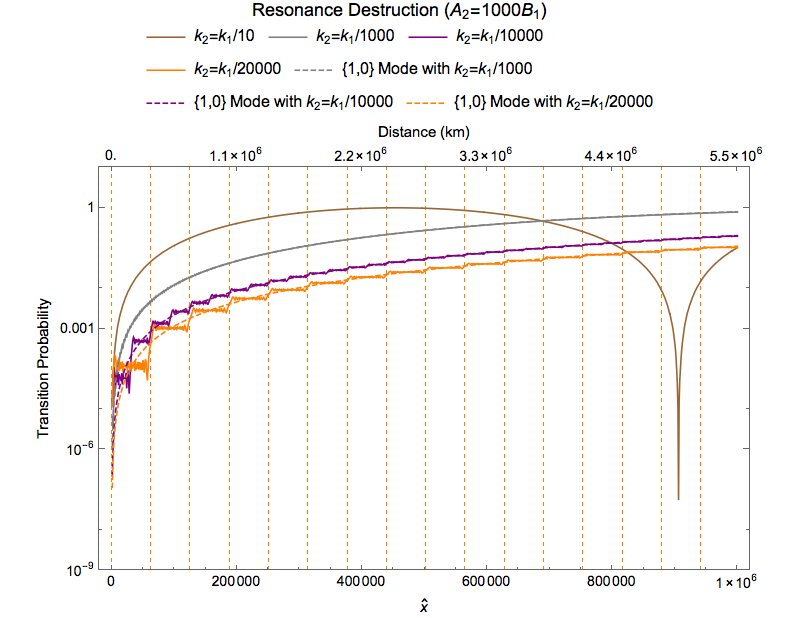
\includegraphics[width=\columnwidth]{assets/interference}
                \caption{.... Remake this fig}
                \label{fig-interference}
\end{figure}








%%%%%%%%%%%%%%%%%%%%%%%%%%%%%%%%%%%%%%%%%%%%%%%%%%%%
%%%%%%%%%  Stimulated Neutrino Oscillations  %%%%%%%%%%%%%%%%%%%
%%%%%%%%%%%%%%%%%%%%%%%%%%%%%%%%%%%%%%%%%%%%%%%%%%%%

\section{\label{sec:jacobi}Parametric Resonance and Rabi oscillation --- Jacobi-Anger expansion}


With the intuition of the Rabi oscillation itself as well as the interference with long wave length mode shown in Sec.~\ref{sec:simple}, we can interpret the transition probabilities of any matter profile more precisely if the system can be exactly decomposed into multiple Rabi oscillations. In this section, we show that the matter effect can be decomposed into superpositions of Rabi oscillations. For a system of single frequency matter perturbation, $\delta \lambda(r) = \lambda_1 \sin(k_1 r)$ in Eq.~(\ref{eq-hamiltonian-bg-matter-basis-general}), we apply an unitary transformation of the form
\begin{equation}
    \mathbf{U} =  \begin{pmatrix} e^{-i \eta (r)} & 0 \\  0 & e^{i \eta (r)}  \end{pmatrix},
    \label{eq-rabi-transformation}
\end{equation}
which is a transformation used in reference \onlinecite{Kneller2006} to remove the diagonal elements of the Hamiltonian. In this work, this transformation is used to remove the varying $\sigma_3$ terms $\delta\lambda(r) \cos 2\theta_{\mathrm m} \sigma_3/2$ in the Hamiltonian, so that the energy gap is fixed in the new basis $\left(\ket{\nu_{\mathrm{r1}}},\ket{\nu_{\mathrm{r2}}}\right)^{\mathrm{T}}$, which is defined as
\begin{equation}
    \begin{pmatrix} \ket{\nu_{\mathrm{r1}}}\\ \ket{\nu_{\mathrm{r2}}} \end{pmatrix} =  \mathbf{U}^\dagger \begin{pmatrix} \ket{\nu_{\mathrm{L}}} \\ \ket{\nu_{\mathrm{H}}} \end{pmatrix}.
    \label{eq-rabi-basis}
\end{equation}
For convenience, we name this unitary transformation Rabi transformation in Eq.~(\ref{eq-rabi-transformation}) as well as the new basis in Eq.~(\ref{eq-rabi-basis}) the Rabi basis. In Rabi basis, we find the Schr\"{o}dinger equation
\begin{widetext}
\begin{equation*}
    \begin{pmatrix}  \frac{\mathrm d\eta}{\mathrm dr}  & 0 \\ 0 & - \frac{\mathrm d\eta}{\mathrm d r}  \end{pmatrix} \begin{pmatrix} \psi_{\mathrm R1} \\ \psi_{\mathrm R2} \end{pmatrix} + \mathrm i \frac{\mathrm d}{\mathrm dr} \begin{pmatrix} \psi_{\mathrm R1} \\ \psi_{\mathrm R2} \end{pmatrix} 
    =
\left[ -\frac{\omega_{\mathrm m} }{2} \sigma_3  + \frac{\delta \lambda}{2} \cos 2\theta_{\mathrm m}  \sigma_3  - \frac{\delta \lambda}{2} \sin 2\theta_{\mathrm m} \begin{pmatrix} 0 & e^{2\mathrm i\eta} \\ e^{-2 \mathrm i\eta } & 0 \end{pmatrix}   \right] \begin{pmatrix} \psi_{\mathrm R1} \\ \psi_{\mathrm R2} \end{pmatrix},
\end{equation*}
\end{widetext}
in which the varying diagonal elements in Hamiltonian can be eliminated by choosing $\eta(x)$ properly, i.e.,
\begin{equation}
    \eta(x) - \eta(0) = - \frac{\omega_{\mathrm{m}}}{2} x + \frac{\cos 2\theta_{\mathrm{m}}}{2} \int_0^x \delta\lambda (\tau) d\tau.
\end{equation}
In Rabi basis, the Schr\"{o}dinger equation becomes
%\begin{widetext}
\begin{equation*}
    i \frac{d}{dx} \begin{pmatrix} \psi_{\mathrm r1} \\ \psi_{\mathrm r2} \end{pmatrix} = \left[ - \frac{\omega_{\mathrm m}}{2} \sigma_3 - \frac{\delta \lambda}{2} \sin 2\theta_m \begin{pmatrix} 0 & e^{2i\eta} \\ e^{-2 i\eta } & 0 \end{pmatrix}\right] \begin{pmatrix} \psi_{\mathrm r1} \\ \psi_{\mathrm r2} \end{pmatrix},
\end{equation*}
%\end{widetext}
where $\eta(x) = - A_1 \cos 2\theta_{\mathrm m} \cos (k_1 x)/(2 k) $ for single frequency matter profile with potential $\delta\lambda(x) = A_1\sin(k_1x)$.  One can easily show that the transition probability between two eigenstates in Rabi basis is the same as the transition probability between two eigenstates in background matter basis.

To make a connection with Rabi oscillation, we apply Jacobi-Anger expansion, which is used in \cite{Kneller2013}, to decompose the $\exp\left( i z \cos\left(\Phi \right) \right)$-like term in Hamiltonian into linear combinations of terms that is proportional to $\exp\left(i n \Phi \right)$, i.e., to decompose spherical waves into plane waves. The final form of Hamiltonian that show the Hamiltonian is a summation of Rabi systems is
%\begin{widetext}
\begin{equation*}
    %H^{(\mathrm{R})} = 
    -\frac{\omega_{\mathrm{m}}}{2} 
    -  \frac{1}{2} \sum_{n=-\infty}^\infty B_n \begin{pmatrix}
    0 &  \Phi_n e^{i (n k_1-\omega_{\mathrm{m}}) x} \\
     \Phi_n^* e^{ - i (n k_1 -\omega_{\mathrm{m}}) x} & 0
    \end{pmatrix},
\end{equation*}
%\end{widetext}
where
\begin{align*}
    B_n &= \tan 2\theta_{\mathrm m} n k_1 J_{n} \left( \frac{A_1}{k_1}\cos 2\theta_{\mathrm m} \right),\\
    \Phi_n &= e^{i\pi (3n/2+1)},
\end{align*}
with $J_n$ standing for the Bessel function.
The constant phase $\Phi_n$ doesn't play any role in the transition probability since it only determines the initial phase of perturbing Hamiltonian vector in the flavor isospin picture.\fbox{More about the picture.} For the same reason, phase in matter profile is not included. As such systems can be graphically represented on a Bloch sphere, the second term in the Hamiltonian is the many driving fields of the system. It can also be derived for arbitrary multi-frequency matter profile,
\begin{equation}
    \lambda(x) = \lambda_0 + \sum_n A_n \sin (n k_n)
\end{equation}
that the Hamiltonian also takes a form of summations of Rabi oscillations,
\begin{widetext}
\begin{equation}
    H^{(\mathrm r)} = -\frac{\omega_{\mathrm m}}{2} - \frac{1}{2} \sum_{n_1=-\infty}^\infty \cdots \sum_{n_N = -\infty}^\infty B_N 
    \begin{pmatrix}
    0 & \Phi_N e^{i\left( \sum_a n_a k_a - \omega_{\mathrm{m}}\right)x} \\
    \Phi_N^* e^{-i\left( \sum_a n_a k_a - \omega_{\mathrm{m}}\right)x} & 0
    \end{pmatrix},
\end{equation}
\end{widetext}
where
\begin{align*}
    B_N &=  \tan 2\theta_{\mathrm m} \left( \sum_a n_a k_a \right) \left( \prod_a J_{n_a}\left( \frac{A_a}{k_a}\cos 2\theta_m \right) \right),\\
    \Phi_N &= e^{i\pi (3\sum_a n_a/2+1)}.
\end{align*}

When the system has one dominate resonance mode and without significant interference between the resonance mode and other modes, all modes off resonance can be dropped without significantly changing the transition probabilities. However, as we have shown previously in Sec.~\ref{sec:simple}, interference might happen between different modes. A qualitative measure should be introduced so that we know what the conditions are for dropping other modes. The following subsections will determine the important modes of the system (i.e., which $n$ to include) and explore the interference between modes hence explain the coincidence presented in the previous sections. For numerical calculations, we use dimensionless quantities which are scaled using the characteristic energy scale $\omega_{\mathrm{m}}$, e.g.,
\begin{align*}
    \hat x &= \omega_{\mathrm{m}}x, \\
    \hat k_1 & = \frac{k_1}{\omega_{\mathrm{m}}}, \\
    \hat A_1 & = \frac{A_1}{\omega_{\mathrm{m}}}, \\
    \hat B_n &= \frac{B_n}{\omega_{\mathrm{m}}}.
\end{align*}

    

\subsection{The Important Factors}


\fbox{
\parbox{0.9\columnwidth}{
\begin{itemize}
            \item Width of resonance $B$
            \item Deviation from exact resonance $g$, called {\bf{detuning}} (value).
            \item Oscillation wavelength of mode (determined by Rabi frequency, which is in turn related to $B$ and $g$ ) compared to size of physical system
\end{itemize}
}}


For illustration purpose, we use single frequency matter profile to demonstrate the important factors in this system. To determine the important modes, the resonance width for each mode which is determined by $B_n$, the deviation from exact resonance (i.e., detuning) which is calculated as $\lvert n k_1 - \omega_{\mathrm{m}} \rvert$, and oscillation wavelength of each mode compared to the size of the physical system should be considered. By utilizing the theory of Rabi oscillation, we know that the oscillation wavelength of each mode is determined by the Rabi frequency $\Omega_n$.

More specifically, we define the resonance quality $Q_n = \lvert B_n/( n k_1 - \omega_{\mathrm{m}}  )\rvert$, which measures how well the resonance is. For exact resonance, $Q_n=0$, while large $Q_n$ says the system is too far away from the resonance of this specific mode. FIG.~\ref{fig-modes-and-detuning} explains the meaning of $Q_n$. Small $Q_n$ modes are the modes that are dramatically important to the system, on the other hand, modes that has much larger oscillation wavelength are not subjected to be considered even though their $Q_n$'s are close to zero, which is due to the fact that such modes have not accumulated much transition probabilities within the size of the physical system.


\begin{figure}[!htbp]
                \centering
                
\includegraphics[width=\columnwidth]{assets/placeholder.jpg}%fig-modes-and-detuning}
                \caption{fig-modes-and-detuning}
                \label{fig-modes-and-detuning}
\end{figure}


\fbox{
\parbox{\columnwidth}{%
FIGS:
\begin{itemize}
    \item Resonance width and transition amplitude? But this is probably something people already know about.
    \item {\bf Width is dropping as n increase. Combine the plot with the limit when $n$ is large.}
    \item Show that only the first mode is important in some situations. And the correction due to higher orders.
\end{itemize}
}
}


Similar quantities are to be considered for multi-frequency matter profile, such as the resonance width of each mode $B_N$, detuning $\lvert \sum_a n_a k_a - \omega_{\mathrm{m}} \rvert$, and Rabi frequency $\Omega_N$, as well as $Q_N =\lvert B_N/( \sum_a n_a k_a - \omega_{\mathrm{m}}  )\rvert$.








\section{\label{conclusions}Conclusions}

%%%% Do not repeat what has been said


\fbox{
\parbox{0.9\columnwidth}{
CONCLUSION PLACEHOLDER
}}



\section{\label{acknowledgement}Acknowledgement}

The first author would like to thank J. Kneller and K. Patton for their help during this research.




%%%%%%%%%%%%%%%%%%%%%%%%%%%%%%%%%%%%%%%%%%
%%%%%%%%%%%%% APPENDIX  %%%%%%%%%%%%%%%%%%
%%%%%%%%%%%%%%%%%%%%%%%%%%%%%%%%%%%%%%%%%%



% \newpage\null\thispagestyle{empty}
% \vspace{20em}
% This page is intentionally left blank
% \newpage


% \clearpage
\appendix
\section{\label{sec:three-bases}Three Bases}

\fbox{Define the three different bases used.}

\section{\label{sec:rabi-oscillations}Rabi Oscillations}


\fbox{
\parbox{0.9\columnwidth}{

\begin{itemize}
\item Derive the transition probability using flavor isospin method.    
\end{itemize}

}
}


The Hamiltonian for Rabi oscillation is
\begin{equation}
    H_{\mathrm R} = - \frac{\omega_{\mathrm R}}{2} \sigma_3 - A_{\mathrm{R}} \cos (k_{\mathrm{R}} x + \phi_{\mathrm{R}}) \sigma_1,
    \label{rabi-oscillation-single-perturbation}
\end{equation}
in which $\omega_{\mathrm R}$ serves as the energy split of the two level system, while $A_{\mathrm{R}}$ and $k_{\mathrm{R}}$ are the strength and frequency of the driving field, respectively. A decomposition of the second term shows that
\begin{align*}
H_{\mathrm R} =& -\frac{\omega_{\mathrm R}}{2}\sigma_3 - \frac{A_{\mathrm{R}} }{2}  \left( \cos(k_{\mathrm{R}}r+\phi_{\mathrm{R}})\sigma_1  - \sin(k_{\mathrm{R}}r+\phi_{\mathrm{R}}) \sigma_2 \right) \nonumber \\
&- \frac{A_{\mathrm{R}} }{2}  \left( \cos(k_{\mathrm{R}}r+\phi_{\mathrm{R}})\sigma_1 + \sin(k_{\mathrm{R}}r+\phi_{\mathrm{R}}) \sigma_2 \right) \\
=& - \frac{\boldsymbol{\sigma}}{2} \cdot (\mathbf{H}_3 + \mathbf{H}_+ + \mathbf{H}_- ) ,
\end{align*}
where $\boldsymbol{\sigma}$ is the the vector of Pauli matrices, and the three vectors are
\begin{align}
    \mathbf{H}_3 = & \begin{pmatrix}
    0 \\ 0 \\ \omega_{\mathrm R}
    \end{pmatrix} \\
    \mathbf{H}_+ = & \begin{pmatrix}
    A_{\mathrm{R}} \cos(k_{\mathrm{R}}r+\phi_{\mathrm{R}}) \\
    - A_{\mathrm{R}} \sin(k_{\mathrm{R}}r+\phi_{\mathrm{R}}) \\
    0
    \end{pmatrix} \\
    \mathbf{H}_- = & \begin{pmatrix}
    A_{\mathrm{R}} \cos(k_{\mathrm{R}}r+\phi_{\mathrm{R}}) \\
    A_{\mathrm{R}} \sin(k_{\mathrm{R}}r+\phi_{\mathrm{R}})  \\
    0
    \end{pmatrix}.
\end{align}

The three vectors are mapped onto a Cartesian coordinate system, so that $\mathbf{H}_3$ is the vector aligned with the third axis, $\mathbf{H}_+$ and $\mathbf{H}_-$ are two rotating vectors in a plane perpendicular to $\mathbf{H}_3$.

Such a system has analytical transition probability from low energy state to high energy state
\begin{equation}
    P(x) = \frac{\left \lvert A_{\mathrm{R}} \right \rvert ^2}{ \Omega_{\mathrm R}^2 } \sin^2 \left( \frac{\Omega_{\mathrm R}}{2} x \right),
    \label{rabi-system-hamiltonian}
\end{equation}
where
\begin{equation}
\Omega_{\mathrm R} = \sqrt{ \lvert A_{\mathrm{R}}\rvert^2 + (k_{\mathrm{R}} - \omega_{\mathrm R})^2 }
\end{equation} is known as Rabi frequency. The detuning, which is defined as $k_{\mathrm{R}} - \omega_{\mathrm R}$, determines how off-resonance the system is, and amplitude of optical field $A_{\mathrm{R}}$ determines the resonance width. The transition probability oscillates with frequency $\Omega_{\mathrm R}$, however, optical field amplitude $A_1$ is the dominate factor for oscillation frequency when the system is close to resonance.





\bibliographystyle{unsrt}
\bibliography{ref.bib} 



%%%%%%%%%%%%%%%%%%%%%%%%%%%%%%%%%%%%%%%%%%
%%%%%%%%%%%%% APPENDIX  %%%%%%%%%%%%%%%%%%
%%%%%%%%%%%%%%%%%%%%%%%%%%%%%%%%%%%%%%%%%%









\end{document}